\documentclass[tikz]{standalone}
\usepackage{ctex}
\usepackage{tikz}
\usepackage{pgfplots}
\pgfplotsset{compat=1.18}   % 使用较新版本语法
\usetikzlibrary{positioning, arrows.meta, intersections, calc, fit, backgrounds}
\usepgfplotslibrary{fillbetween}  % 用于填充区域

\begin{document}
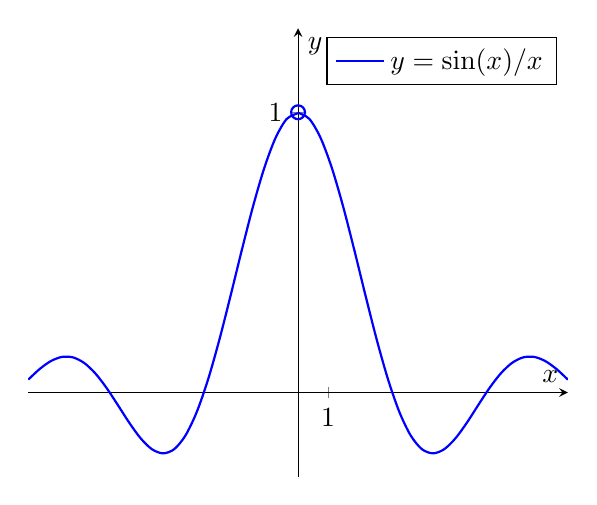
\begin{tikzpicture}
    \begin{axis}[
            % width=0.45\textwidth,
            axis lines = middle,
            xlabel = $x$, ylabel = $y$,
            xmin = -9, xmax = 9,
            ymin = -0.3, ymax = 1.3,   % 缩小 y 范围，突出变化
            xtick = {0,1},
            xticklabels = {0,1},
            ytick = {1},
            yticklabels = {1},
            % axis equal = true,       % 去掉或注释掉
            clip = true,
            every axis plot post/.append style={thick}
        ]
        \addplot[blue, domain=-9:-0.005, smooth] {sin(deg(x))/x};
        \addplot[blue, domain=0.005:9, smooth] {sin(deg(x))/x};
        \addplot[blue, only marks, mark=o, mark size=2.5pt] coordinates {(0,1)};
        \addlegendentry{$y=\sin(x)/x$}
    \end{axis}
\end{tikzpicture}
\end{document}